\section{Las siguientes gráficas corresponden a la solución $x(t)$, $x(0) = x'(0) = 0$ de una de las ecuaciones siguientes que se indican a continuación. Determina a qué ecuación corresponde cada gráfica}
\\
\\
\begin{itemize}
    \item[a)] $x'' + 15x = cos\left(4t \right)$
        \\
        \begin{figure}[h]
            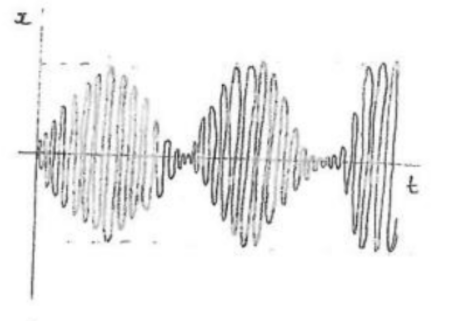
\includegraphics[scale = 1.2]{Ejercicios/Imágenes/E13_EDO_a.PNG}
            \centering
        \end{figure}
    \item[b)] $x'' + \sqrt{5}x' + 16x = cos\left(4t \right)$
        \\
        \begin{figure}[h]
            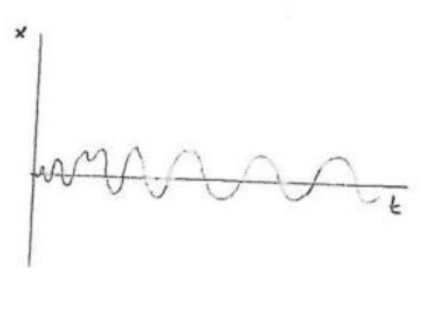
\includegraphics[scale = 1.2]{Ejercicios/Imágenes/E13_EDO_b.PNG}
            \centering
        \end{figure}
    \item[c)] $x'' + 16x = \frac{1}{2}cos\left(4t \right)$
        \\
        \begin{figure}[h]
            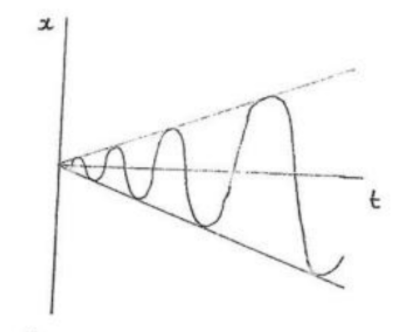
\includegraphics[scale = 1.2]{Ejercicios/Imágenes/E13_EDO_c.PNG}
            \centering
        \end{figure}
    \item[d)] $x'' + 16x = 10$
        \\
        \begin{figure}[h]
            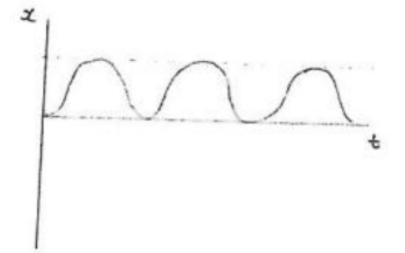
\includegraphics[scale = 1.2]{Ejercicios/Imágenes/E13_EDO_d.PNG}
            \centering
        \end{figure}
    \item[e)] $x'' + 16x = 5cos\left(3t \right)$
        \\
        \begin{figure}[h]
            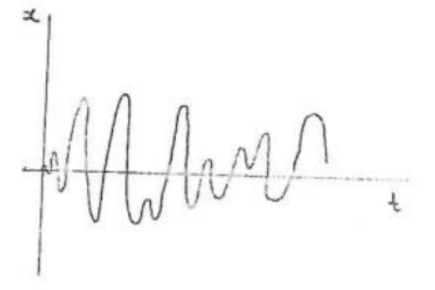
\includegraphics[scale = 1.2]{Ejercicios/Imágenes/E13_EDO_e.PNG}
            \centering
        \end{figure}
\end{itemize}